\chapter{REALM Demonstration}
% Main Gist 
% - Demonstrate OpenMC problem with REALM. 
% Structure 
% - realm demonstration of OpenMC Coupling for a toy problem. 
In this chapter, I demonstrate using \gls{REALM} to apply genetic algorithms 
to maximize $k_{eff}$ in a single \gls{AHTR} fuel slab.  

\section{Straightened AHTR Fuel Slab}
\subsection{Problem Definition}
The objective of this demonstration is to explore how inhomogeneous fuel 
distributions impact $k_{eff}$ compared to homogenous fuel distributions that 
are customary in most reactor designs. 
The reactor core explored is a straightened slab from the \gls{FHR} benchmark's
\gls{AHTR} design.
Figure \ref{fig:straightened_slab} illustrates the straightened fuel slab. 
\begin{figure}[]
    \centering
    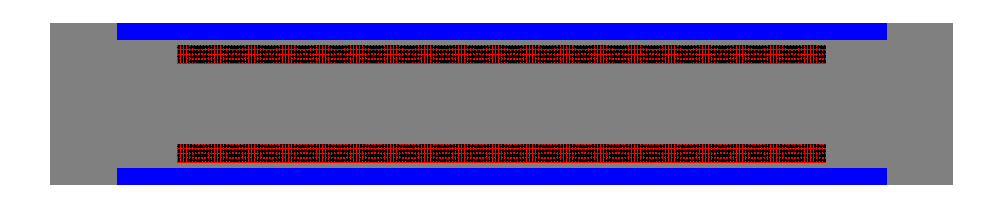
\includegraphics[width=\linewidth]{straightened_slab.png}
    \raggedright
    \resizebox{0.3\textwidth}{!}{
        \hspace{1cm}
        \fbox{\begin{tabular}{ll}
            \textcolor{fhrblue}{$\blacksquare$} & FLiBe \\
            \textcolor{fhrgrey}{$\blacksquare$} & Graphite (Fuel Plank)\\
            \textcolor{fhrred}{$\blacksquare$} & Graphite (Fuel Stripe) \\
            \textcolor{fhrblack}{$\blacksquare$} & TRISO particle 

            \end{tabular}}}
    \caption{Straightened \acrfull{AHTR} fuel slab.}
    \label{fig:straightened_slab}
\end{figure}
The slab has dimensions of $27.1 \times 3.25 \times 1.85\ cm^3$
with periodic boundary conditions in the x and y directions and reflective 
boundary conditions in the z direction. 
The materials are the same as in the \gls{FHR} benchmark, with the exception 
of the homogenization of each \gls{TRISO} particle's four outer layers: 
porous carbon buffer, inner pyrolytic carbon, silicon carbide layer, and the 
outer pyrolitic carbon. 
The \gls{TRISO} particles' dimensions remain the same.
The $k_{eff}$ for this original straighted \gls{AHTR} configuration is 
$1.38625 \pm 0.00109$. 

The \gls{REALM} optimization problem's objective is to maximize the slab's 
$k_{eff}$, by varying the \gls{TRISO} particle packing fraction across the slab,
while keeping total \gls{TRISO} particle total packing fraction constant at 0.0979. 
This total packing fraction is consistent with the original straightened slab with 
TRISO particles in fuel stripes (Figure \ref{fig:straightened_slab}). 
The slab is divided into ten slices along the x axis between the \gls{FLiBe} and 
graphite buffers resulting in ten $2.31 \times 2.55 \times 1.85\ cm^3$ slices. 
The \gls{TRISO} particle packing fraction's distribution across slices is 
governed by a sine distribution: 
\begin{align}
    PF(x) &= (a\ sin(bx + c) + 2) \times NF\\
    \intertext{where}
    PF & \mbox{packing fraction} \nonumber \\ 
    a &= \mbox{amplitude, peak deviation of the function from zero} \nonumber \\
    b &= \mbox{angular frequency, rate of change of the function argument } [\frac{radians}{s}] \nonumber \\
    c &= \mbox{phase, specifies (in radians) where in its cycle the oscillation is at t = 0.} \nonumber \\
    x &= \mbox{midpoint value for each slice} \nonumber \\
    NF &= \mbox{Normalization factor} \nonumber
\end{align}
The sine distribution's value at each of the ten x-slices' midpoints are collected and 
normalized by the total packing fraction to ensure that there is a consistent 
amount of \gls{TRISO} particles in the slab. 
Thus, for a packing fraction distribution of 
$PF(x) = (0.5\ sin(\frac{\pi}{3}x + \pi) + 2)  \times NF$. 
The packing fraction for the ten slices are 0.103, 0.120, 0.049, 0.138, 
0.076, 0.081, 0.136, 0.048, 0.125, 0.098, respectively. 
Figure \ref{fig:triso_distribution} shows a plot of this sine distribution, highlights 
the packing fraction at the respective midpoints, and an xy view of the slab
with packing fraction varying based on this sine distribution. 
\begin{figure}[]
    \centering
    \makebox[\textwidth][c]{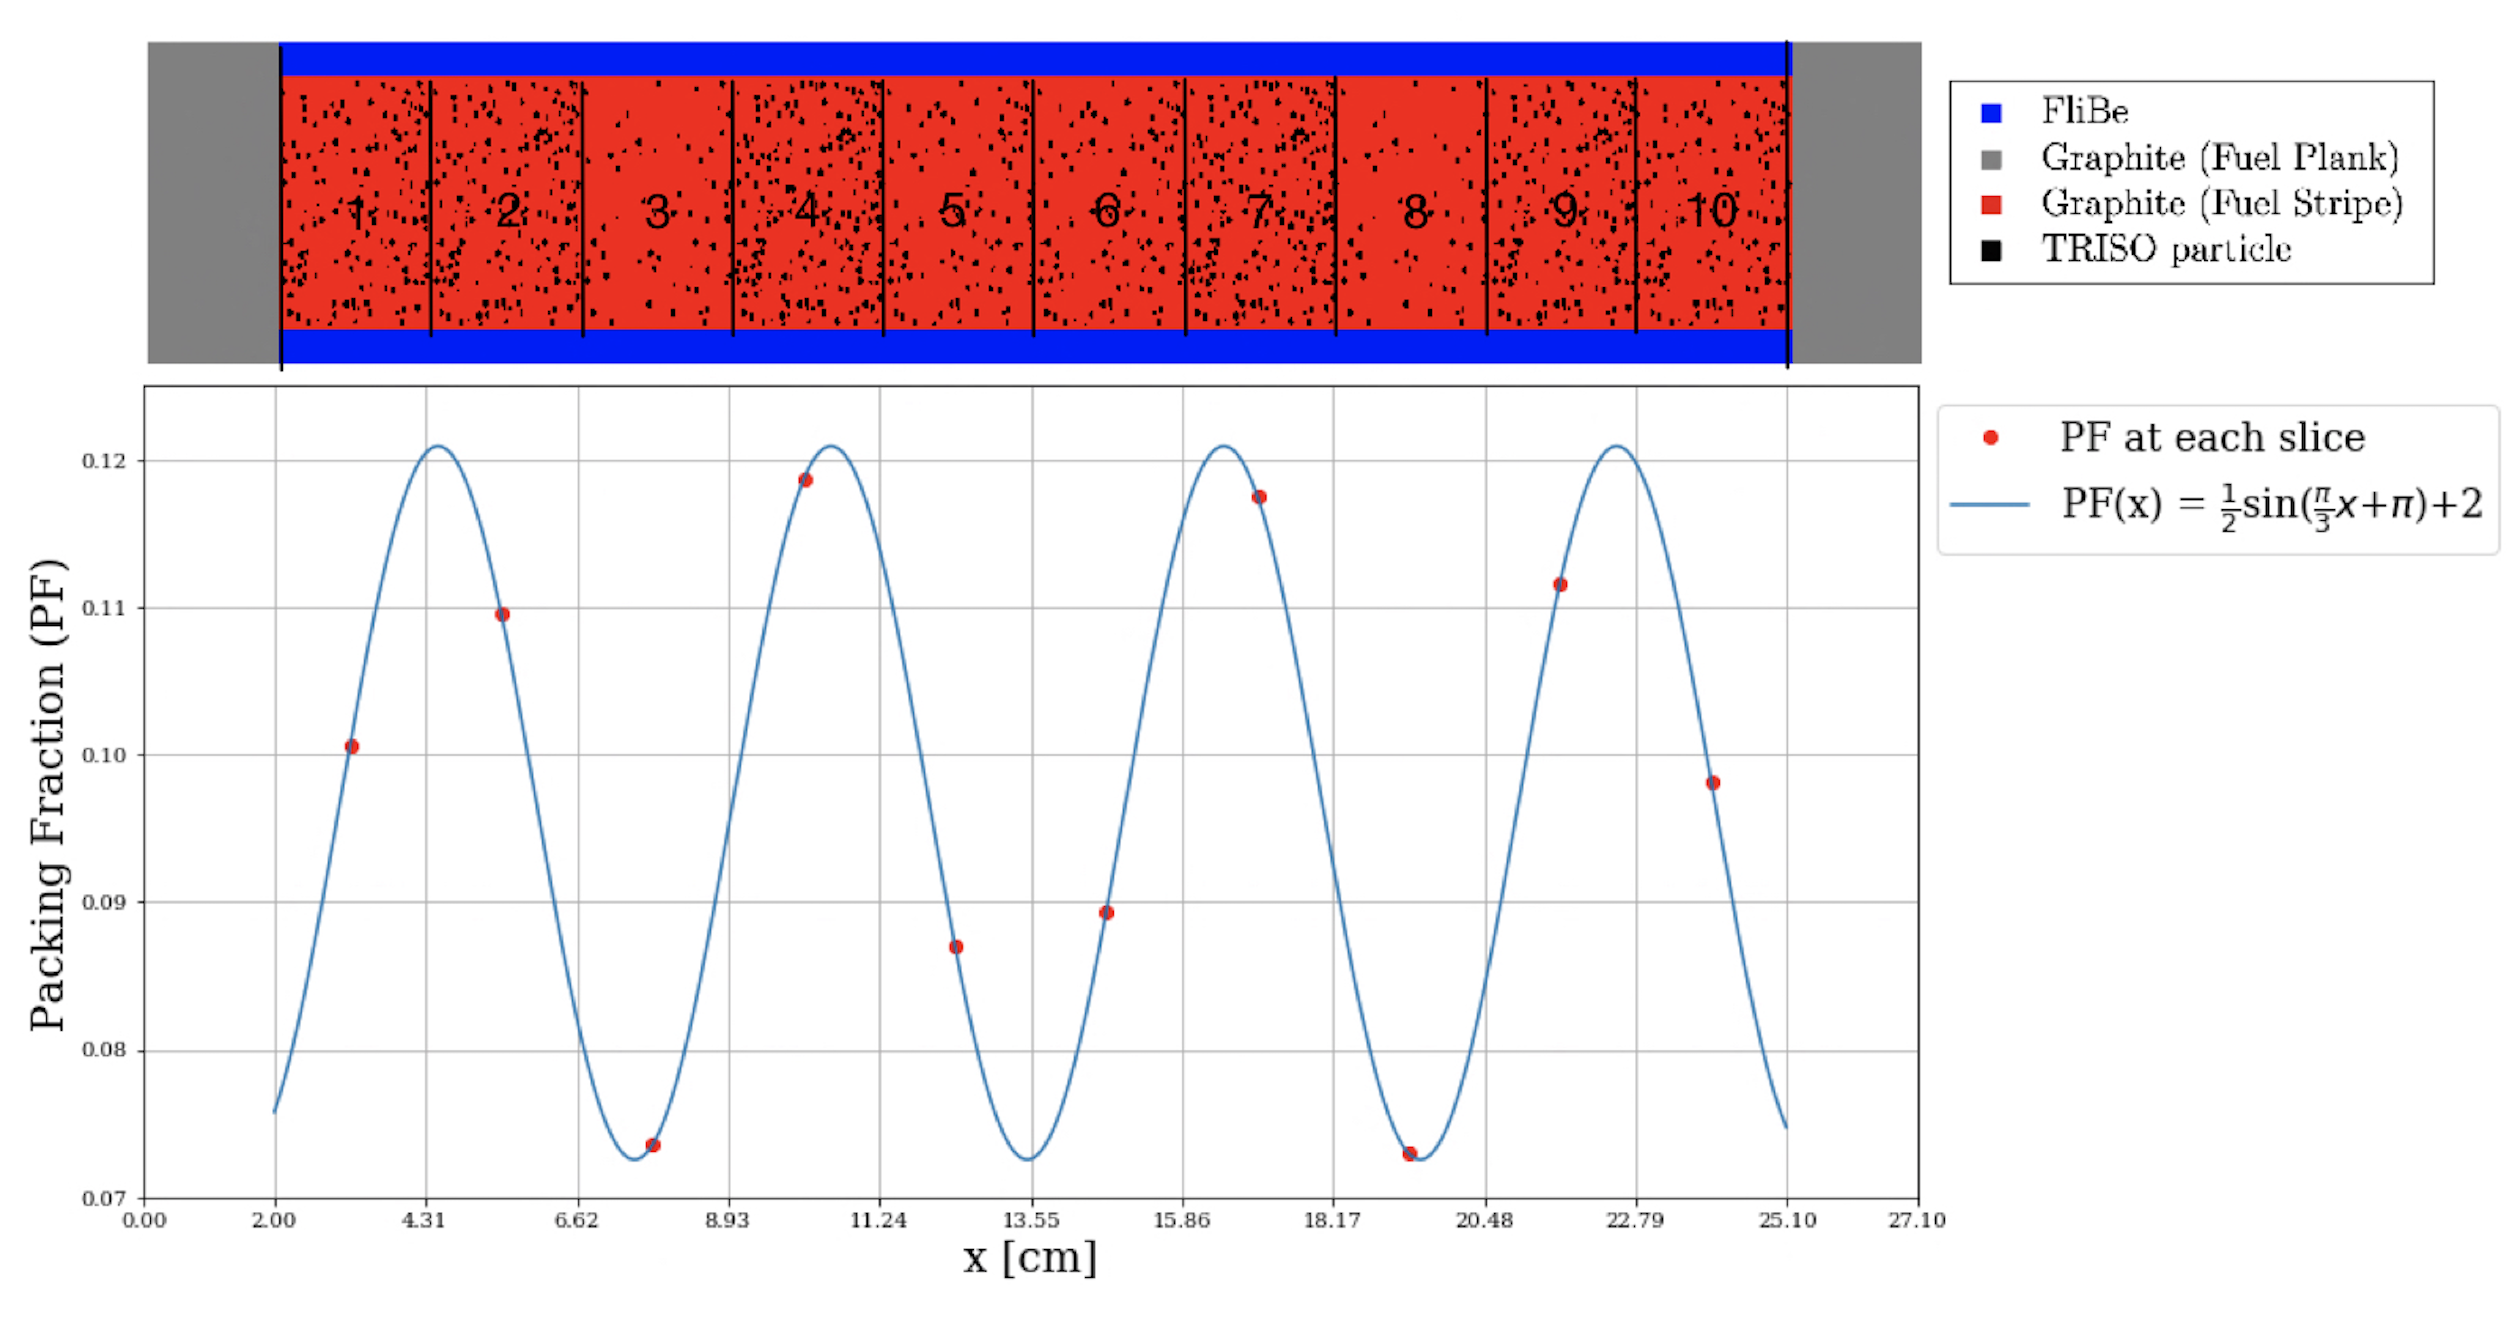
\includegraphics[width=1.1\linewidth]{triso_distribution_sine.png}} 
    \caption{Below: $PF(x) = (0.5\ sin(\frac{\pi}{3}x + \pi) + 2)  \times NF$ 
    sine distribution with red points indicating the packing fraction at each slice. 
    Above: Straightened \acrlong{AHTR} fuel slab with varying \gls{TRISO} particle 
    distribution across ten slices based on the sine distribution. }
    \label{fig:triso_distribution}
\end{figure}

In REALM, a genetic algorithm varies the $a$, $b$ and $c$ variables to find a combination 
that produces a packing fraction distribution that maximizes the $k_{eff}$ in 
the slab. 
The upper and lower bounds of $a$, $b$ and $c$ are: 
\begin{itemize}
    \item 0 $<$ $a$ $<$ 2 
    \item 0 $<$ $b$ $<$ $\frac{\pi}{2}$
    \item 0 $<$ $c$ $<$ $2\pi$
\end{itemize}
The $a$ variable bounds were selected to keep the sine distribution from falling 
below zero. $b$ and $c$ variable bounds are large enough to allow the genetic 
algorithm to explore various sine distributions. 
The OpenMC evaluator calculates $k_{eff}$. 
Each OpenMC simulation is run with 80 active cycles, 20 inactive cycles, and 
8000 particles to reach an uncertainty of approximately 130pcm. 
Figure \ref{fig:realm-input-simple} shows the REALM input file for this 
genetic algorithm optimization problem. 
\texttt{ahtr\_slab\_openmc.py} is the template OpenMC script that accepts 
$a$, $b$ and $c$ from REALM as described in Chapter \ref{chap:realm}. 
\begin{figure}[]
    \begin{minted}[
        frame=lines,
        framesep=2mm,
        baselinestretch=1.2,
        fontsize=\footnotesize,
        linenos
        ]{json}
        {
            "control_variables": {
                "a": {"min": 0.0, "max": 2.0},
                "b": {"min": 0.0, "max": 1.57},
                "c": {"min": 0.0, "max": 6.28},
            },
            "evaluators": {
                "openmc": {
                    "input_script": "ahtr_slab_openmc.py",
                    "inputs": ["a", "b", "c"],
                    "outputs": ["keff"],
                    "keep_files": false,
                }
            },
            "constraints": {"keff": {"operator": [">="], "constrained_val": [1.0]}},
            "algorithm": {
                "objective": "max",
                "optimized_variable": "keff",
                "pop_size": 60,
                "generations": 10,
                "mutation_probability": 0.23,
                "mating_probability": 0.46,
                "selection_operator": {"operator": "selTournament", "k": 15, "tournsize": 5},
                "mutation_operator": {
                    "operator": "mutPolynomialBounded",
                    "eta": 0.23,
                    "indpb": 0.23,
                },
                "mating_operator": {"operator": "cxBlend", "alpha": 0.46},
            },
        }
        
    \end{minted}
    \caption{\acrfull{REALM} JSON input file to maximize $k_{eff}$ in the 
    straightened \acrfull{AHTR} fuel slab by varying packing fraction distribution 
    with control variables, $a$, $b$, $c$.}
    \label{fig:realm-input-simple}
\end{figure}

\subsection{Hyperparameter Search}
REALM's input file allows the user to define the genetic algorithm's 
hyperparameters. 
A good hyperparameter set is able to guide the optimization process by 
balancing exploitation and exploration to find an optimal solution more quickly 
and accurately. 
Finding a good set of hyperparameters requires a trial and error process. 

I performed the hyperparameter search with a coarse-to-fine random sampling scheme, 
whose advantages were previously discussed in Section \ref{sec:balance}.
The hyperparameters varied include: population size, number of generations, 
mutation probability, mating probability, selection operator, selection operator's 
k value, selection operator's tournament size, mutation operator, and mating 
operator.  
I started with 25 coarse experiments and fine tuned the hyperparameters
with 15 more experiments. 
For each genetic algorithm experiment, I hold the number of OpenMC evaluations 
constant at 600.
The population size and number of generations are correlated by the number of 
evaluations. 
I randomly sample population size and use the following equation to calculate 
number of generations: 
\begin{align}
    \mbox{no. of generations} &= \frac{\mbox{no. of evaluations}}{\mbox{population size} }
\end{align}
Table \ref{tab:hyperparameter_search} shows the lower and upper bounds used 
for random sampling of each hyperparameter. 
\begin{table}[]
    \centering
    \onehalfspacing
    \caption{Hyperparameters}
	\label{tab:hyperparameter_search}
    \footnotesize
    \begin{tabular}{p{4cm}lp{3.4cm}p{3.4cm}p{3.4cm}}
    \hline 
    \textbf{Hyperparameter}& \textbf{Type} & \textbf{Coarse Search Bounds} & \textbf{Fine Search 1 Bounds} & \textbf{Fine Search 2 Bounds} \\
    \hline
    Experiments & - & 0 to 24 & 24 to 34 & 35 to 39 \\ 
    \hline
    Population size (pop) & Continuous & 10 $<$ x $<$ 100 & 20 $<$ x $<$ 60 & 60 \\ 
    Mutation probability & Continuous & 0.1 $<$ x $<$ 0.4 & 0.2 $<$ x $<$ 0.4& 0.2 $<$ x $<$ 0.3\\
    Mating probability & Continuous & 0.1 $<$ x $<$ 0.6 &  0.1 $<$ x $<$ 0.3 &  0.45 $<$ x $<$ 0.6\\
    Selection operator & Discrete & \texttt{SelTournament}, \texttt{SelBest}, \texttt{SelNSGA2} & \texttt{SelTournament}, \texttt{SelBest}, \texttt{SelNSGA2}& \texttt{SelTournament}\\
    Selection individuals & Continuous & $\frac{1}{3}pop$ $<$ x $<$ $\frac{2}{3}pop$ & $\frac{1}{3}pop$ $<$ x $<$ $\frac{2}{3}pop$ & 15\\
    Selection tournament size (only for SelTournament) & Continuous & 2 $<$ x $<$ 8 &2 $<$ x $<$ 8&5\\
    Mutation Operator & Discrete & \texttt{mutPolynomialBounded} &\texttt{mutPolynomialBounded}&\texttt{mutPolynomialBounded}\\
    Mating Operator & Discrete& \texttt{cxOnePoint}, \texttt{cxUniform}, \texttt{cxBlend} &\texttt{cxOnePoint}, \texttt{cxUniform}, \texttt{cxBlend}&\texttt{cxOnePoint}, \texttt{cxBlend}\\ 
    \hline
    \end{tabular}
\end{table}

The objective of the initial 25 coarse experiments is to narrow down the 
hyperparameters to find a narrower set of optimal hyperparameter bounds that 
produce higher average $k_{eff}$ values in each experiment's final generation. 
Figure \ref{fig:hyperparameter_sens} shows the hyperparameters' plotted against 
each other with a third color dimension of the average $k_{eff}$ value in each 
experiment's final generation. 
The lighter the scatter point is, the larger the final population's 
average $k_{eff}$ value is, thus the better the hyperparameter set. 
\begin{figure}[]
    \centering
    \makebox[\textwidth][c]{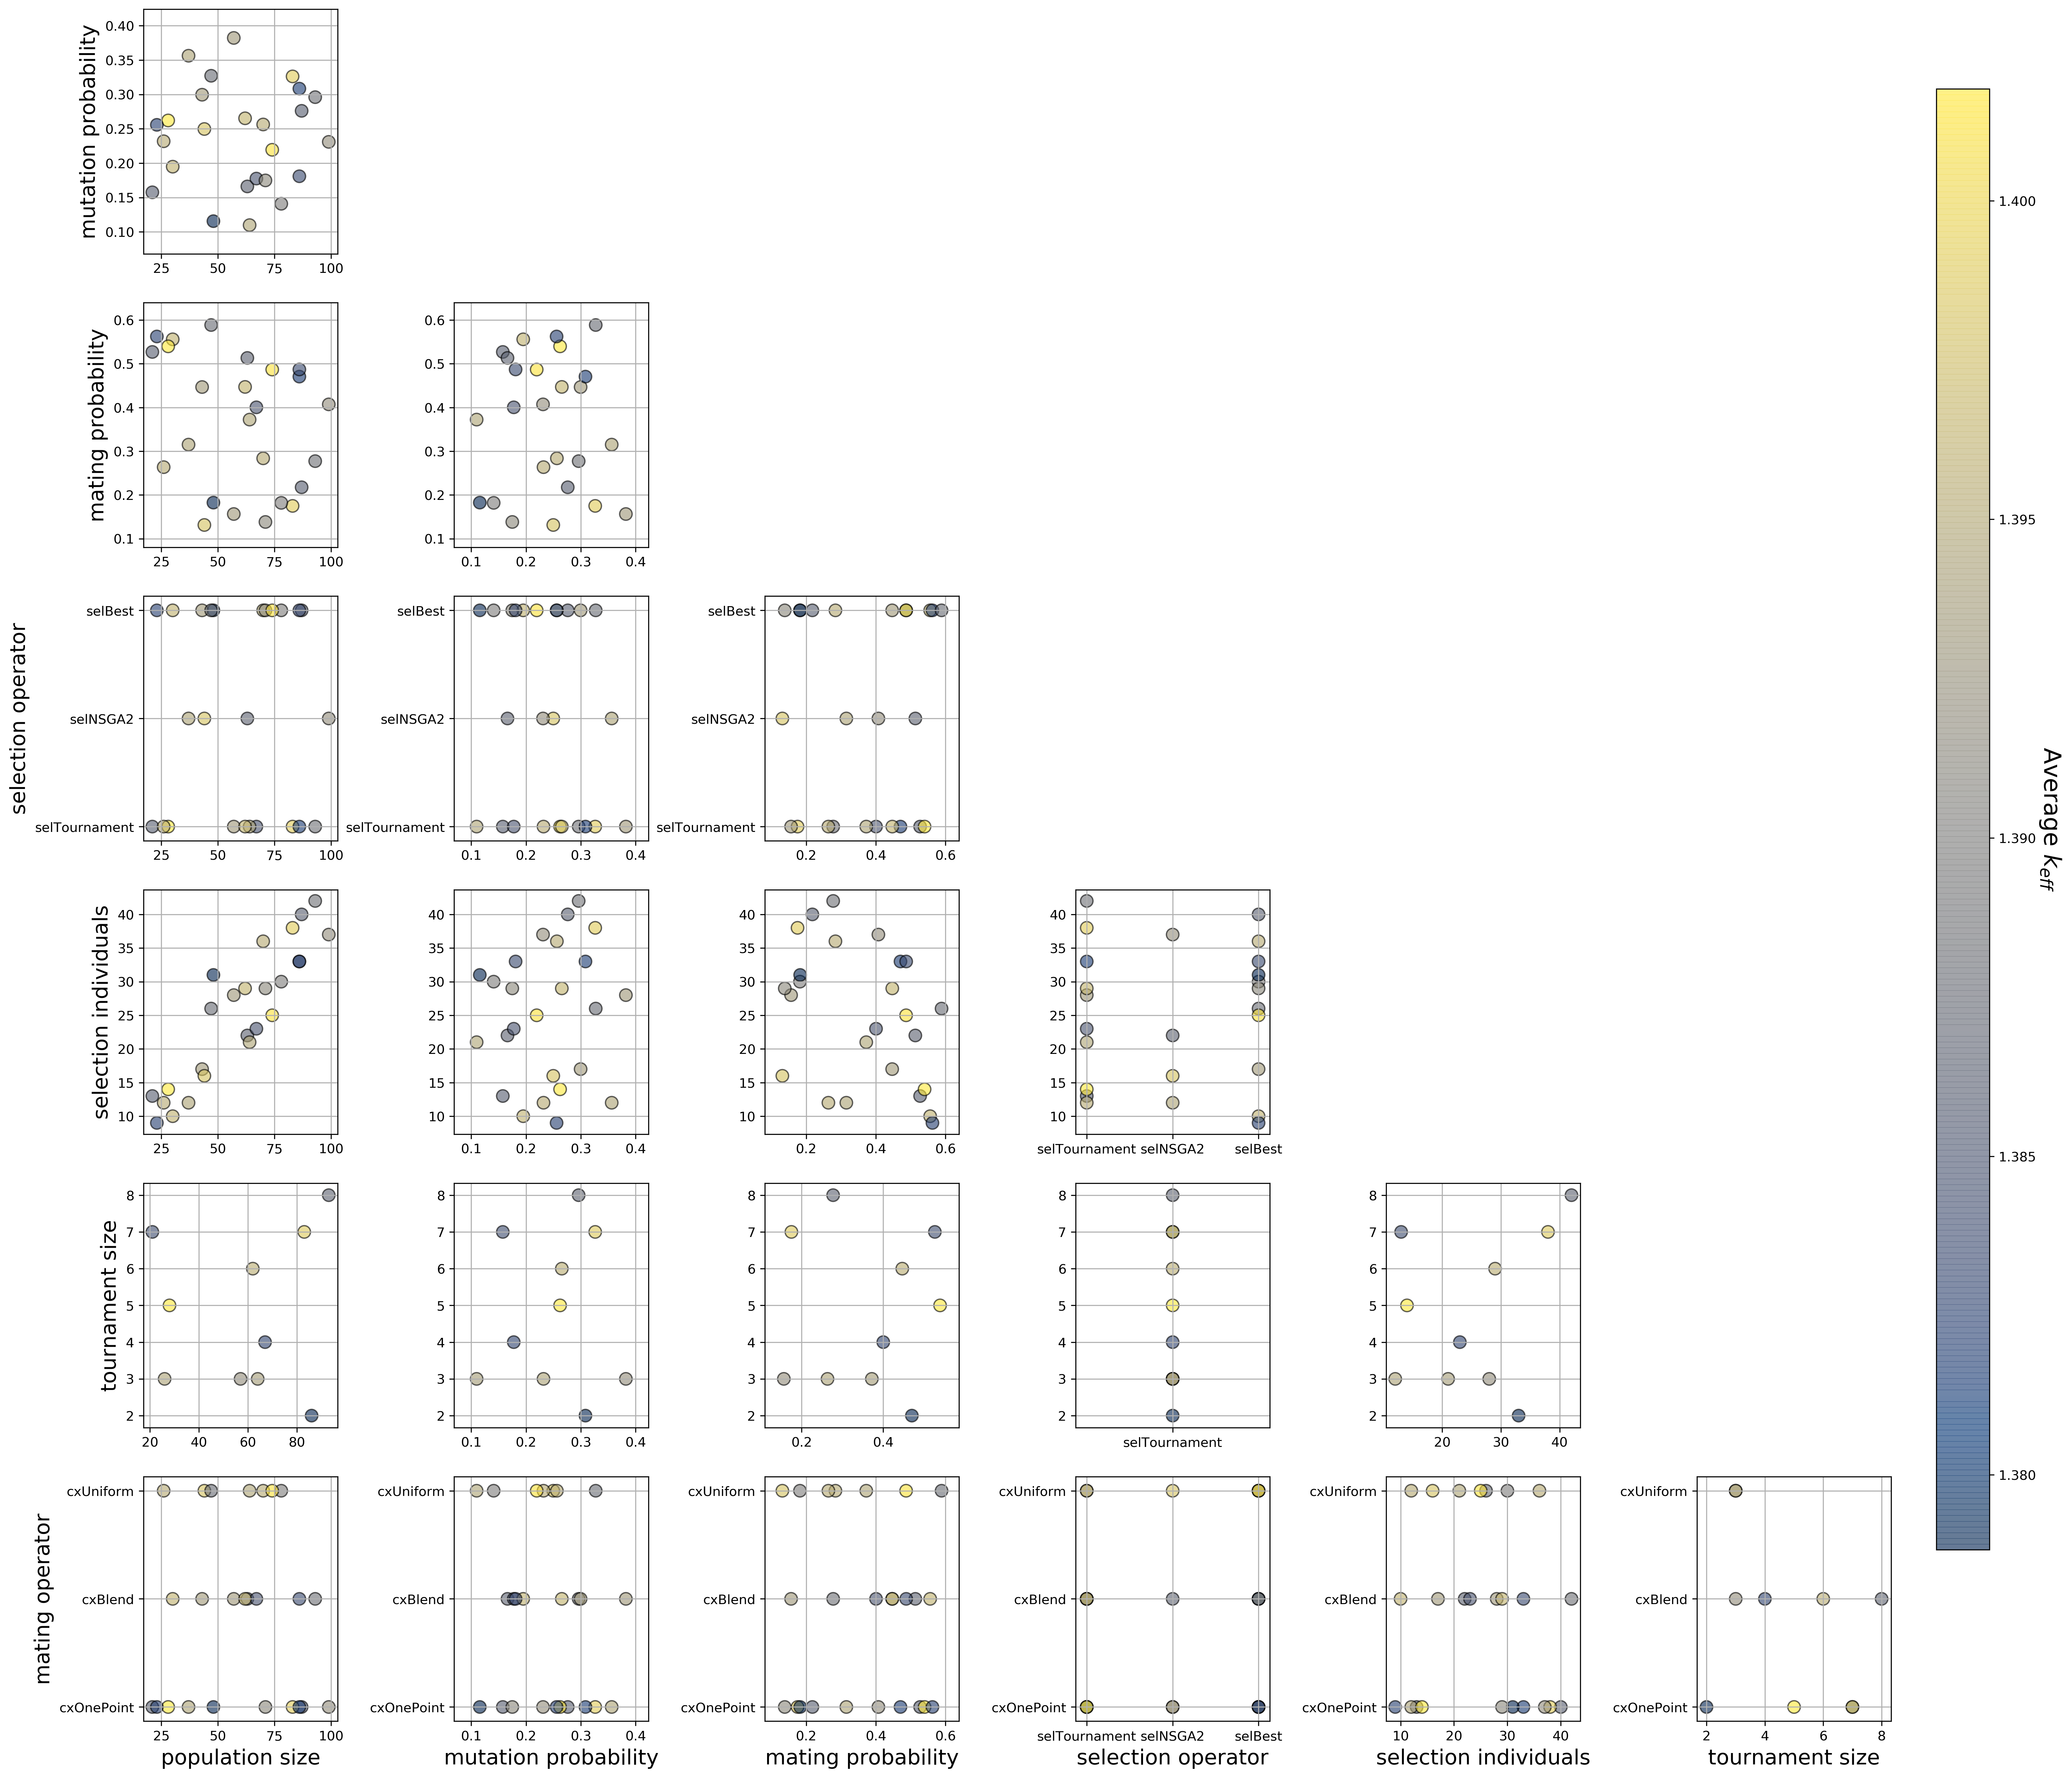
\includegraphics[width=1.3\linewidth]{hyperparameter_sens.png}} 
    \caption{Coarse hyperparameters search's results. Hyperparameter values are plotted 
    against each other with a third dimension of each experiment's final population's 
    average $k_{eff}$ indicated by each scatter point's color.}
    \label{fig:hyperparameter_sens}
\end{figure}
The hyperparameters are plotted against each other to visualize interdependence 
between hyperparameters. 
From the coarse hyperparameter search, the trends that stood out to me were: 
\begin{itemize}
    \item Mutation probability has larger $k_{eff ave}$ between 0.2 and 0.4. 
    \item Mating probability has larger $k_{eff ave}$ when between 0.1 and 0.3. 
    \item Population size has larger $k_{eff ave}$ when between 20 and 60. 
\end{itemize}
There is also not much interdependence between hyperparameters. 

Next, I proceeded to the fine search. 
From Figure \ref{fig:hyperparameter_sens}, I narrowed down population size, 
mutation probability, and mating probability bounds, as shown in Table 
\ref{tab:hyperparameter_search}'s \textit{Fine Search 1 Bounds} column. 
I did not see any significant trends in the other hyperparameters so I chose 
to leave them as is. 
I ran 10 more experiments (25 to 34) with sampling hyperparameters from 
the \textit{Fine Search 1 Bounds}. 
From these results, I conducted a second fine search with 5 experiments 
(35 to 39) with further tuned hyperparameter bounds as shown in Table 
\ref{tab:hyperparameter_search}'s \textit{Fine Search 2 Bounds} column. 
Figure \ref{fig:input_hyperparameters_sens} shows the relationship between 
hyperparameter values and $a$,$b$,$c$ input parameters, final generation 
$k_{eff max}$, and final generation $k_{eff ave}$. 
The coarse experiments' scatter points are $50\%$ transparent, while the fine 
experiments' scatter point are opaque. 
\begin{figure}[]
    \centering
    \makebox[\textwidth][c]{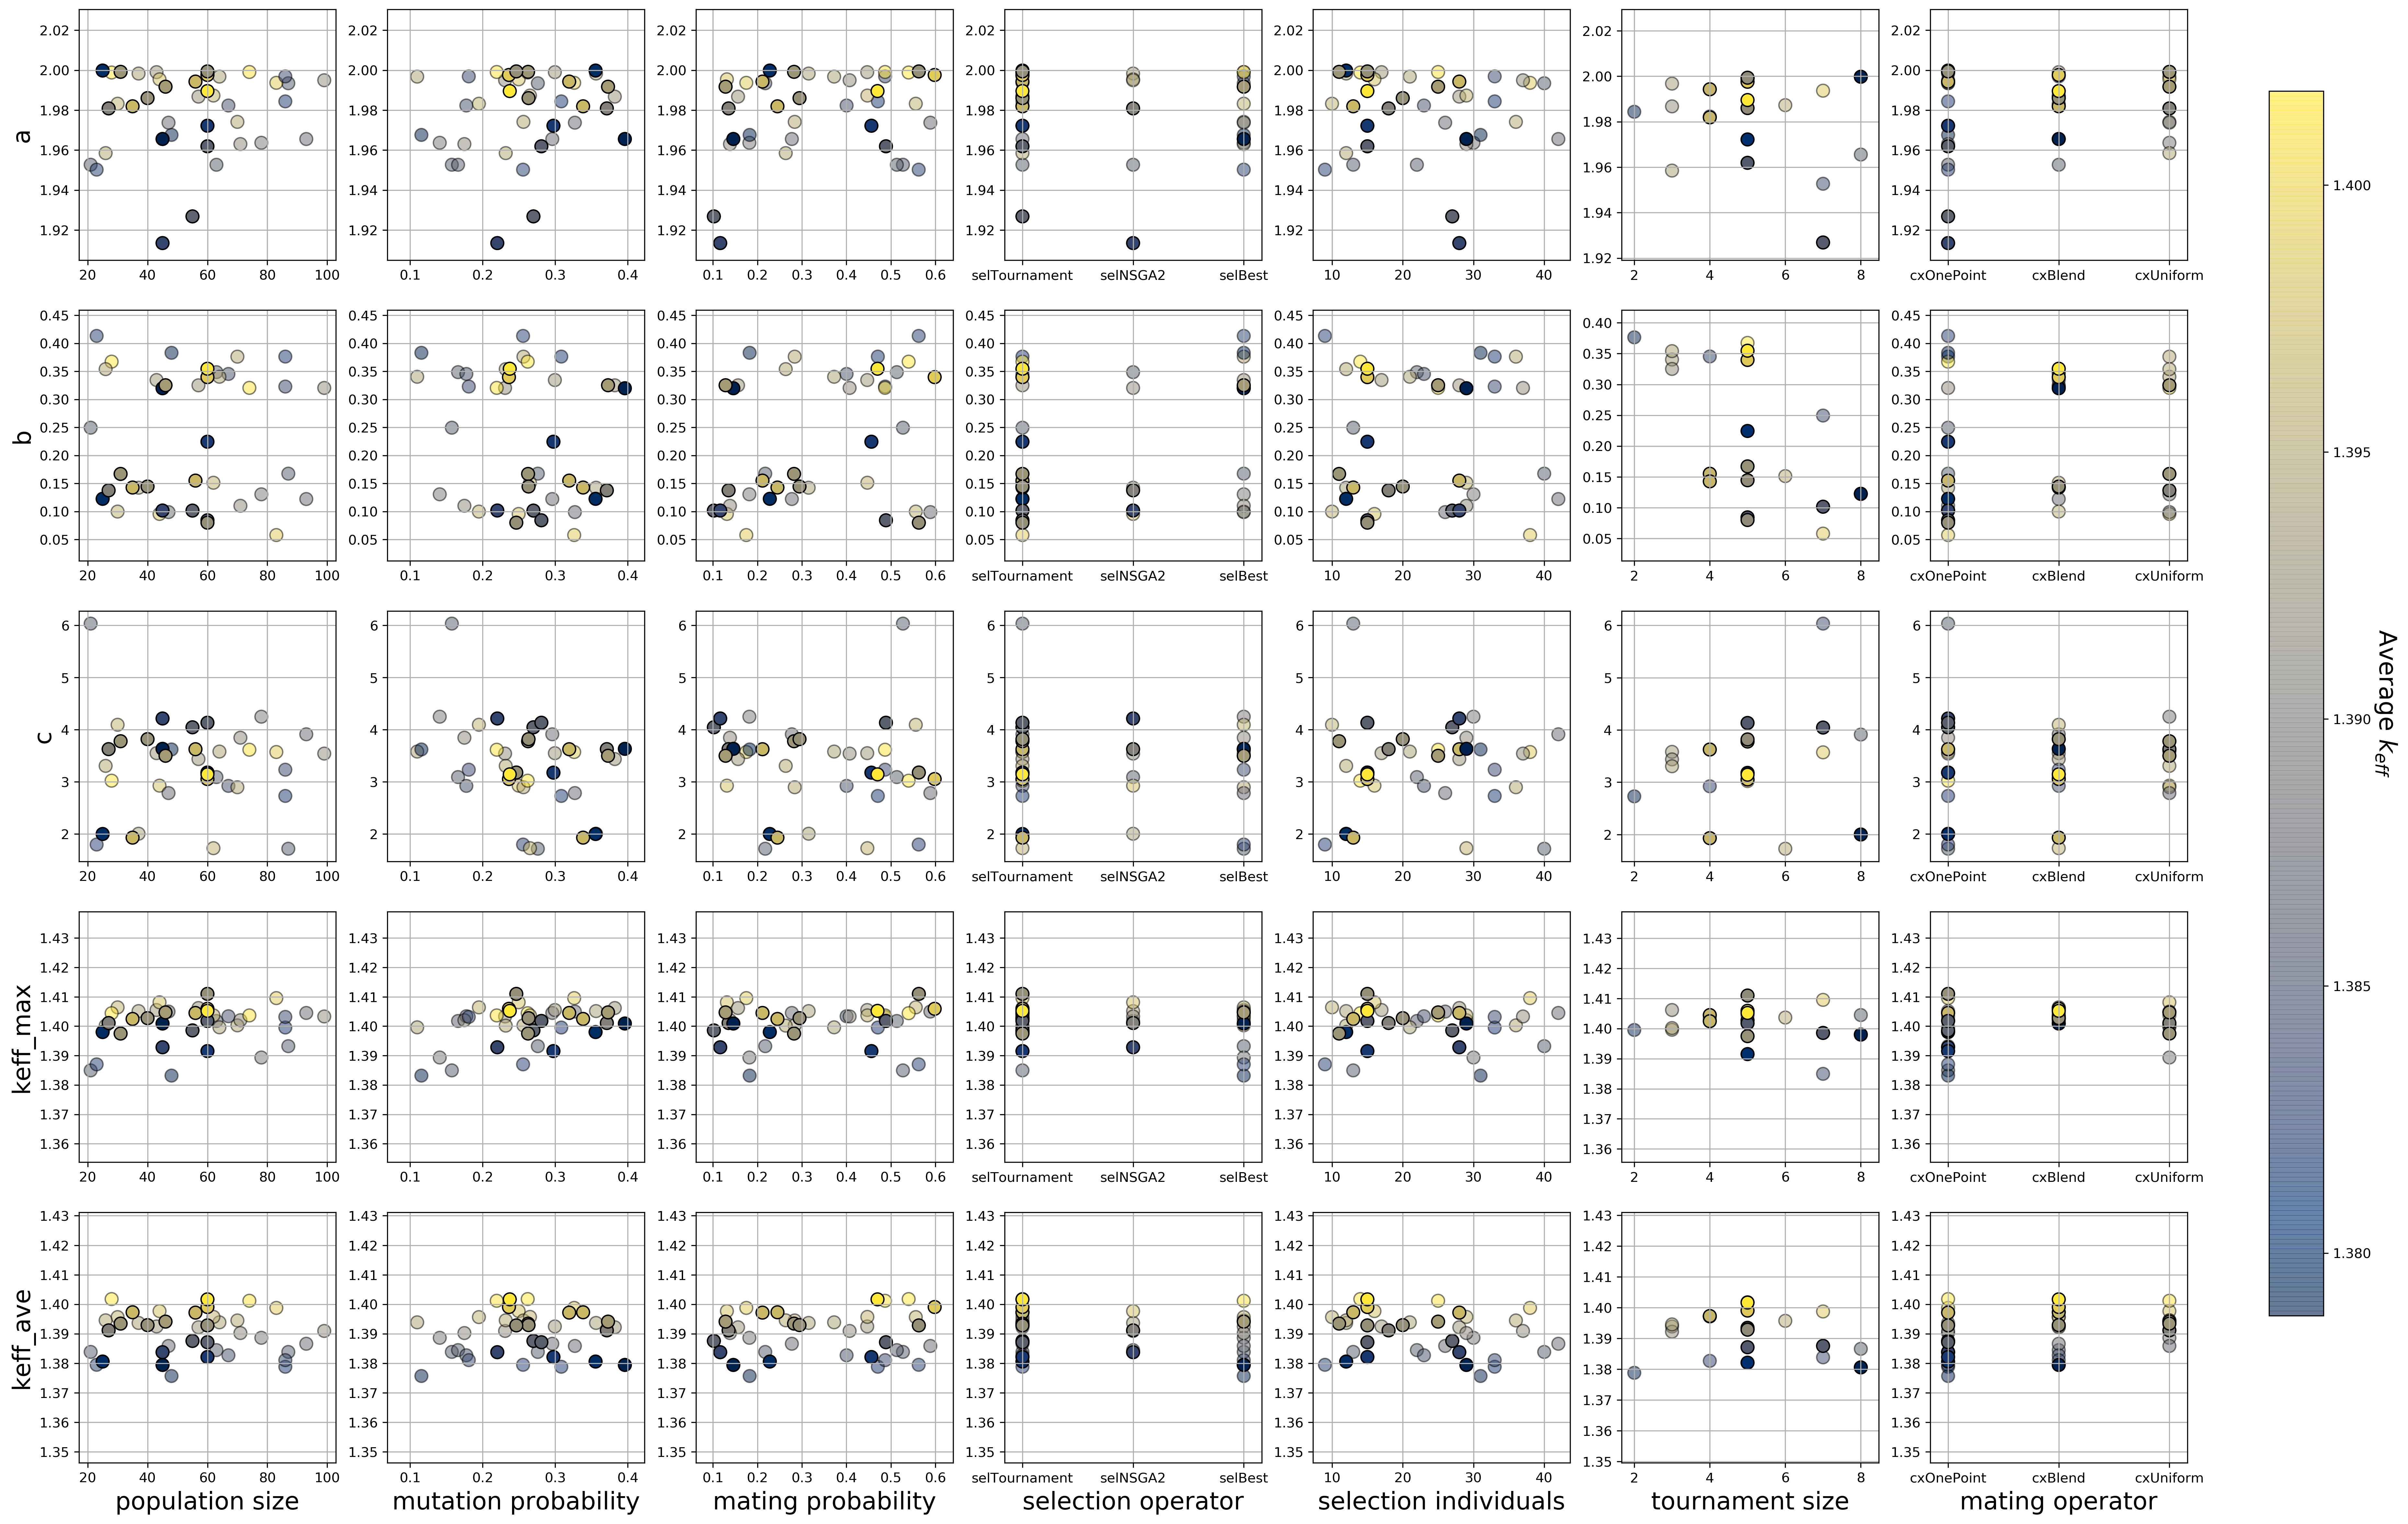
\includegraphics[width=1.3\linewidth]{input_hyperparameters_sens.png}} 
    \caption{Fine hyperparameters search's results. Hyperparameters are plotted 
    against a,b,c input parameters, each experiment's final generation
    $k_{eff max}$, and final generation $k_{eff ave}$ with a third dimension of 
    each experiment's final population's average $k_{eff}$ indicated by each 
    scatter point's color.}
    \label{fig:input_hyperparameters_sens}
\end{figure}

Table \ref{tab:topfive} shows the hyperparameters for the five experiments 
with the highest final generation $k_{eff ave}$.
\begin{table}[]
    \centering
    \onehalfspacing
    \caption{Input and Output Parameters}
	\label{tab:topfive}
    \footnotesize
    \makebox[\textwidth][c]{\begin{tabular}{p{3cm}p{3cm}p{3cm}p{3cm}p{3cm}p{3cm}}
    \hline 
    \textbf{Input/Output Parameters}& \textbf{Experiment 6} & \textbf{Experiment 15} & \textbf{Experiment 24} & \textbf{Experiment 36} & \textbf{Experiment 39}\\
    \hline 
    $k_{eff ave}$ & 1.39876 &1.40175&1.40118&1.39906&1.40165\\ 
    $k_{eff max}$ & 1.40954 &1.40440&1.40365&1.40590&1.40519\\ 
    a & 1.993&1.998&1.999&1.997&1.989\\
    b & 0.057&0.367&0.320&0.339&0.354\\ 
    c & 3.571&3.022&3.615&3.053&3.143\\
    \hline
    \textbf{Hyperparameter}& &&&&\\
    Population size & 83 & 28&74&60&60\\ 
    Generations &8&22&9&10&10 \\
    Mutation probability & 0.32 &0.26&0.21&0.23&0.23\\
    Mating probability & 0.17 &0.53&0.48&0.59&0.46\\
    Selection operator & \texttt{selTournament} &\texttt{selTournament}&\texttt{selBest}&\texttt{selTournament}&\texttt{selTournament}\\
    Selection individuals & 38 &14&25&15&15\\
    Selection tournament size & 7 &5&-&5&5\\
    Mutation Operator & \texttt{mutPolynomial} \texttt{Bounded}&\texttt{mutPolynomial} \texttt{Bounded}&\texttt{mutPolynomial} \texttt{Bounded}&\texttt{mutPolynomial} \texttt{Bounded}&\texttt{mutPolynomial} \texttt{Bounded}\\
    Mating Operator & \texttt{cxOnePoint} &\texttt{cxOnePoint}&\texttt{cxUniform}&\texttt{cxBlend}&\texttt{cxBlend}\\ 
    \hline
    \end{tabular}}
\end{table}
Figure \ref{fig:topfiveplot} shows the packing fraction distributions that 
produced the $k_{eff max}$ from each of the top five experiments. 
\begin{figure}[]
    \centering
    \makebox[\textwidth][c]{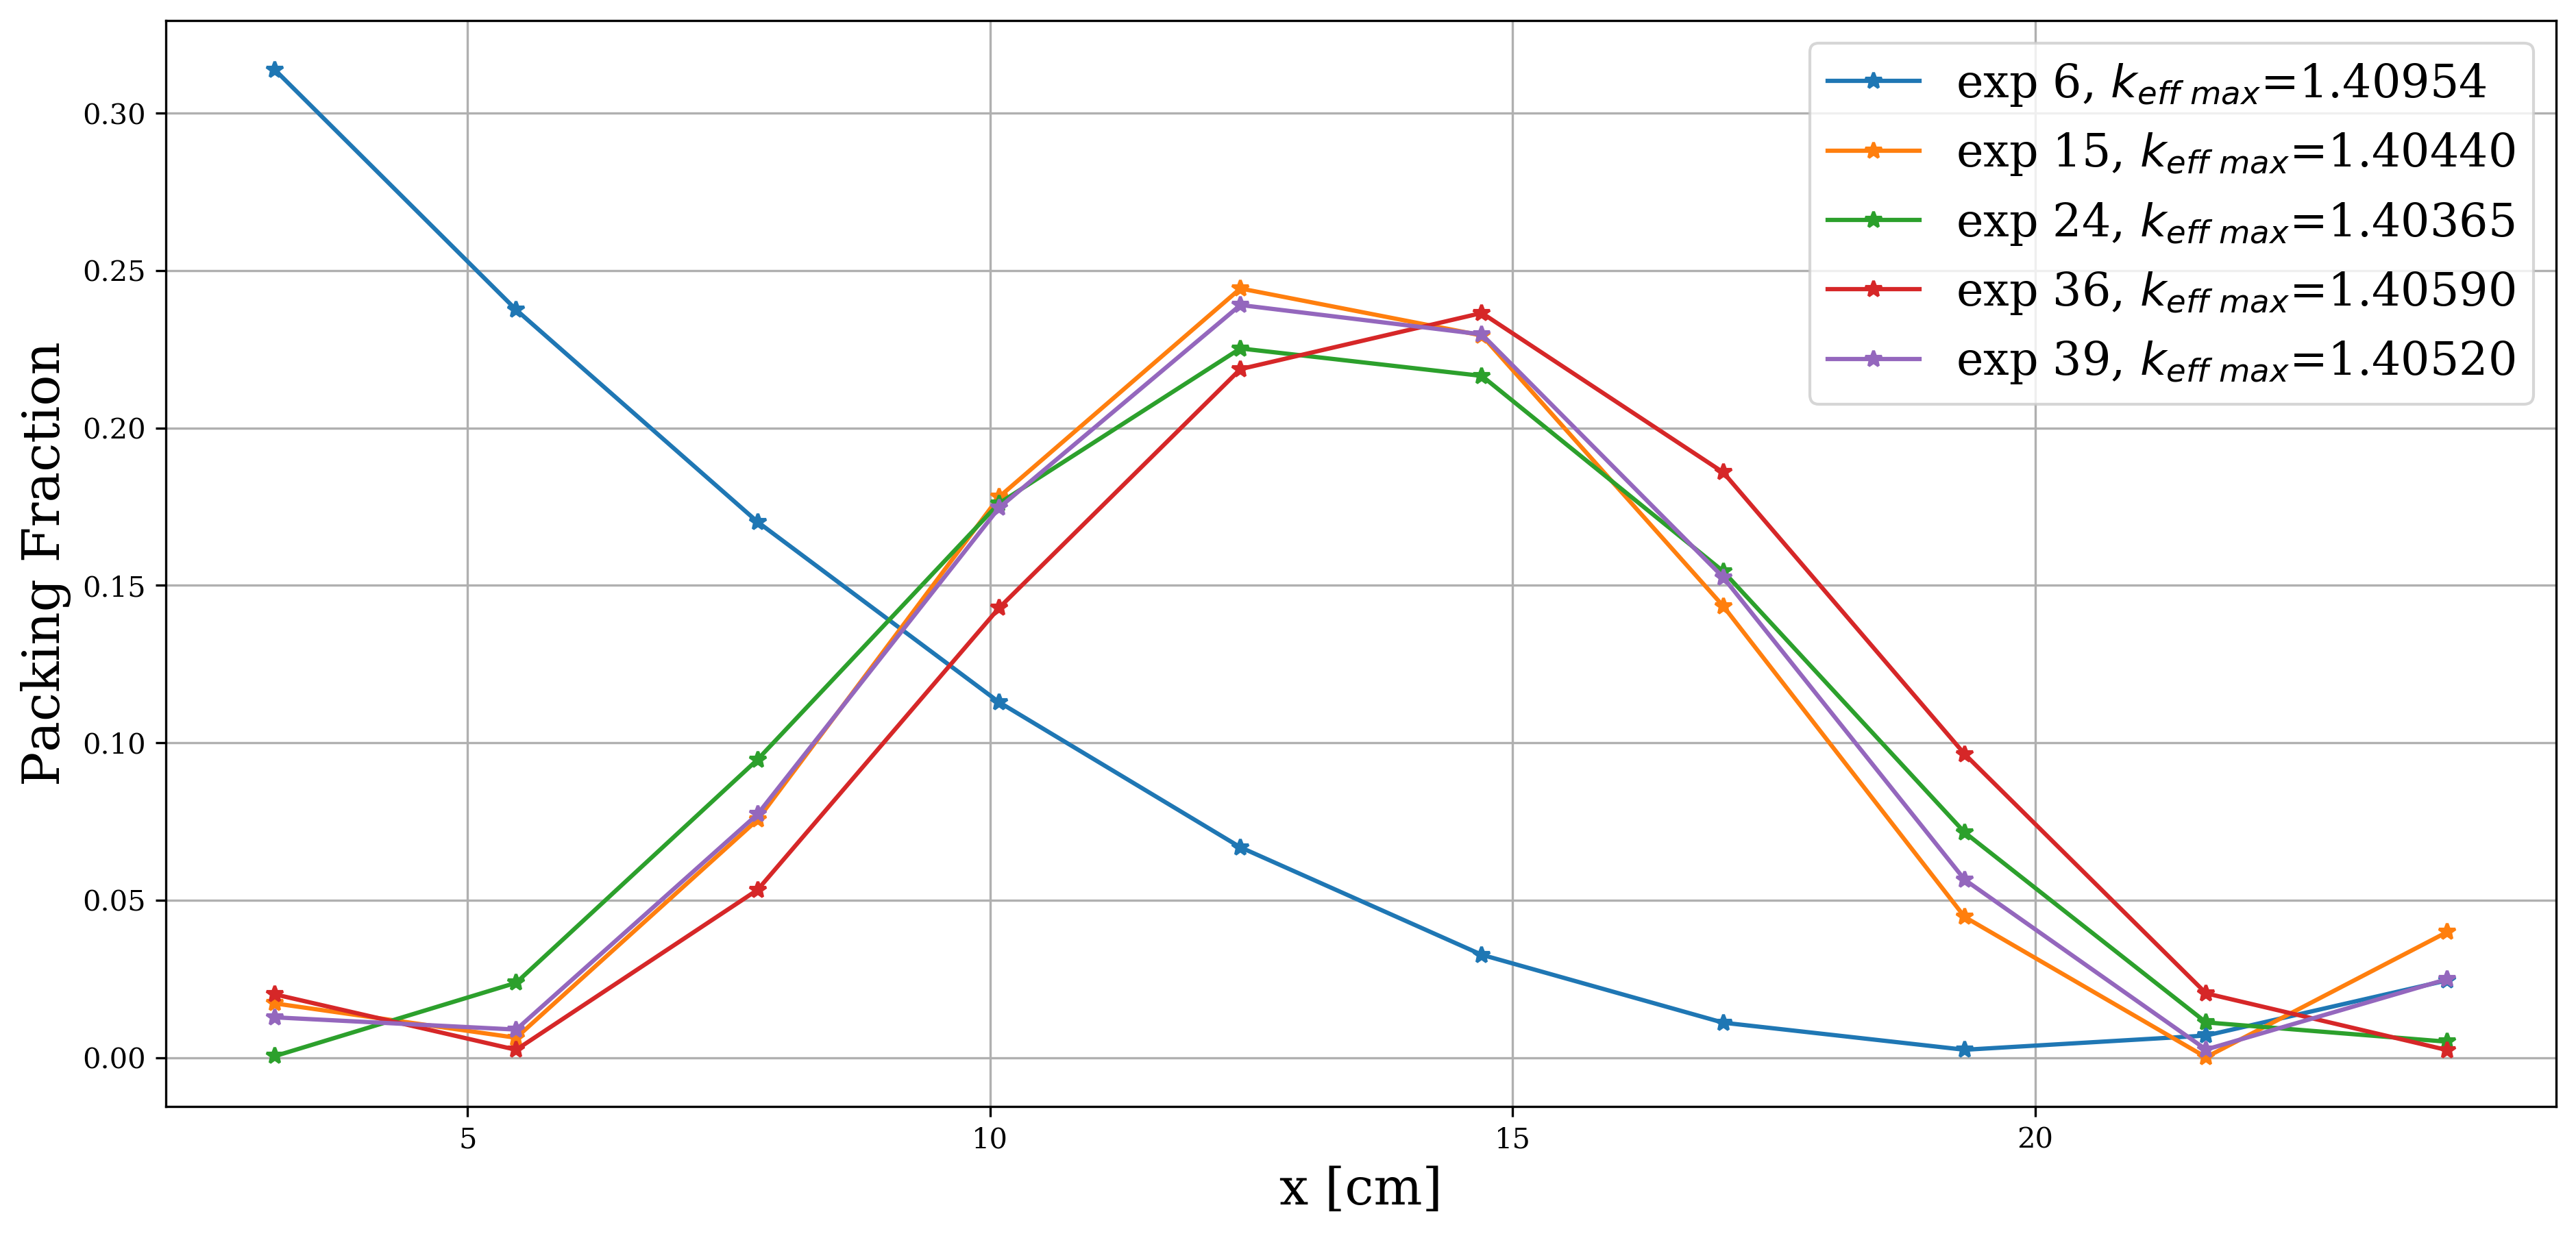
\includegraphics[width=1\linewidth]{topfive_plot.png}} 
    \caption{}
    \label{fig:topfiveplot}
\end{figure}
Four experiments had similar distributions of packing fraction peaking at approximately 
0.23 in the centre of the slab, while one experiment had an exponential-looking 
distribution with peak packing fraction of 0.31 at side of the slab.
This demonstrates the robustness of the genetic algorithms to find similar solutions with 
different hyperparameters. 

\subsection{Results for best hyperparameter set}
I define the best-performing hyperparameter set as the experiment that produces 
the highest final generation $k_{eff ave}$. 
The best performing set of hyperparameters are from the final 
\textit{Fine Search 2} and is experiment 39 in Table \ref{tab:topfive}
with centre-peaking packing fraction distribution with $k_{eff max} = 1.40519$. 
Experiment 39's $k_{eff max}$ is $\sim2000$pcm larger than the original 
straighted \gls{AHTR} configuration's $k_{eff}$. 
Figure \ref{fig:triso_distribution_sine_39} shows the packing fraction distribution 
that produced $k_{eff max} = 1.40519$. 
\begin{figure}[]
    \centering
    \makebox[\textwidth][c]{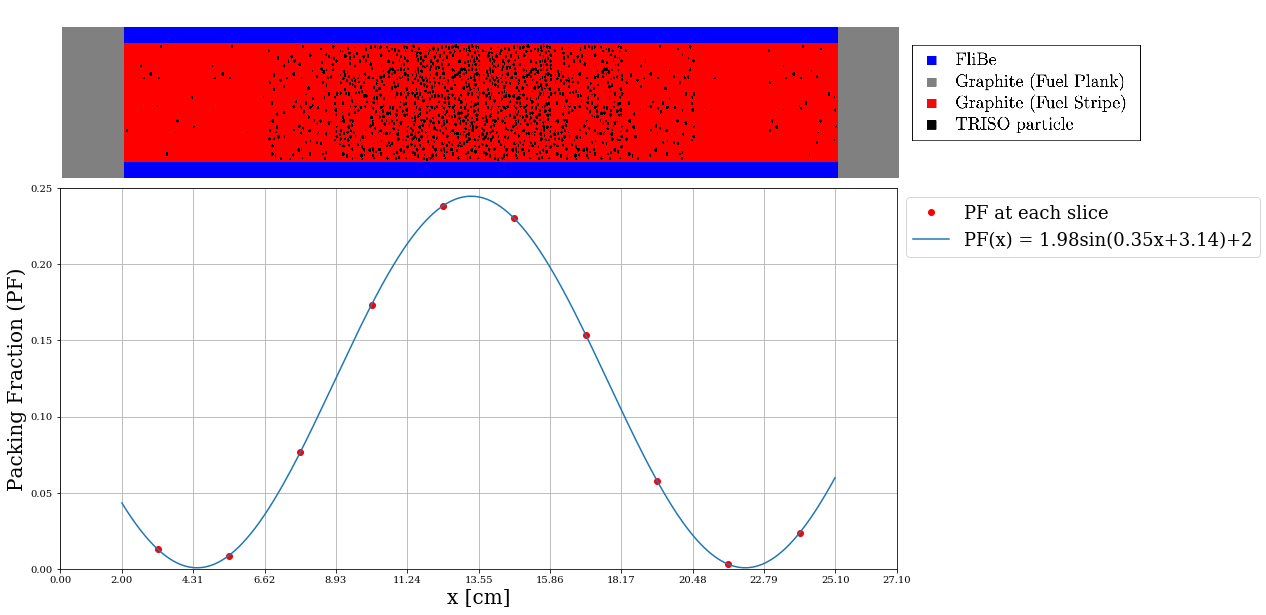
\includegraphics[width=1.1\linewidth]{triso_distribution_sine_39.png}} 
    \caption{Experiment 39 packing distribution that produced $k_{eff max} = 1.40519$. 
    Below: $PF(x) = (1.98\ sin(0.35x+3.14)+2)  \times NF$ sine distribution with 
    red points indicating the packing fraction at each slice. 
    Above: Straightened \acrlong{AHTR} fuel slab with varying \gls{TRISO} particle 
    distribution across ten slices based on the sine distribution. }
    \label{fig:triso_distribution_sine_39}
\end{figure}

Figure \ref{fig:keff_conv_39} and \ref{fig:pf_39} show the evolution of $k_{eff}$ 
and packing fraction distribution through each generation of the best performing 
39$^{th}$ experiment, respectively. 
\begin{figure}[]
    \centering
    \begin{subfigure}{\textwidth}
    \makebox[\textwidth][c]{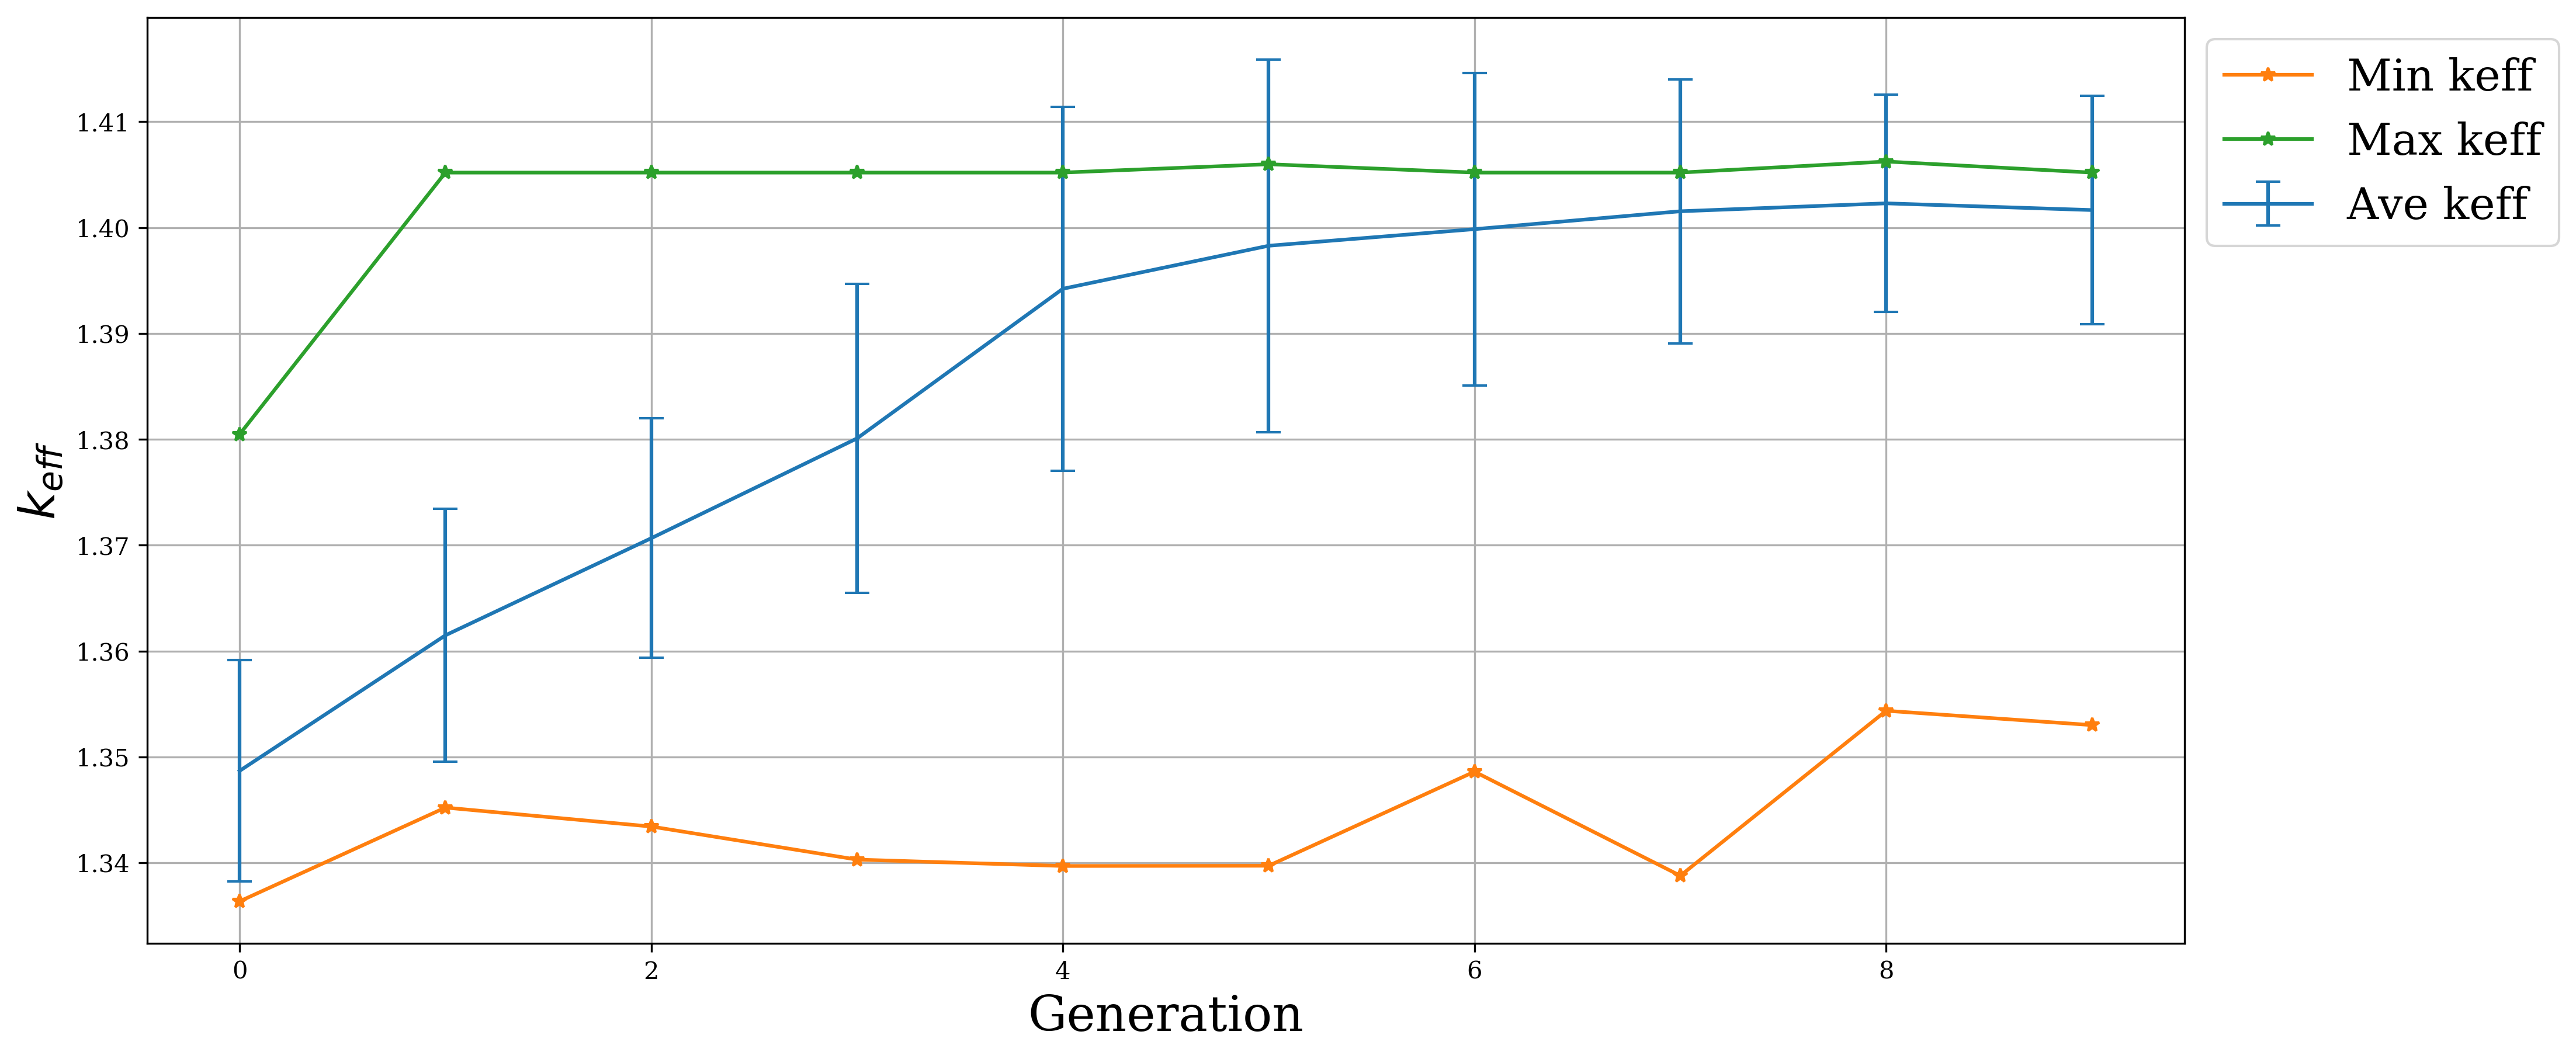
\includegraphics[width=1.1\linewidth]{keff_conv_39.png}} 
    \caption{Minimum, average, and maximum $k_{eff}$ values evolution.}
    \label{fig:keff_conv_39}
    \end{subfigure}
    \begin{subfigure}{\textwidth}
        \makebox[\textwidth][c]{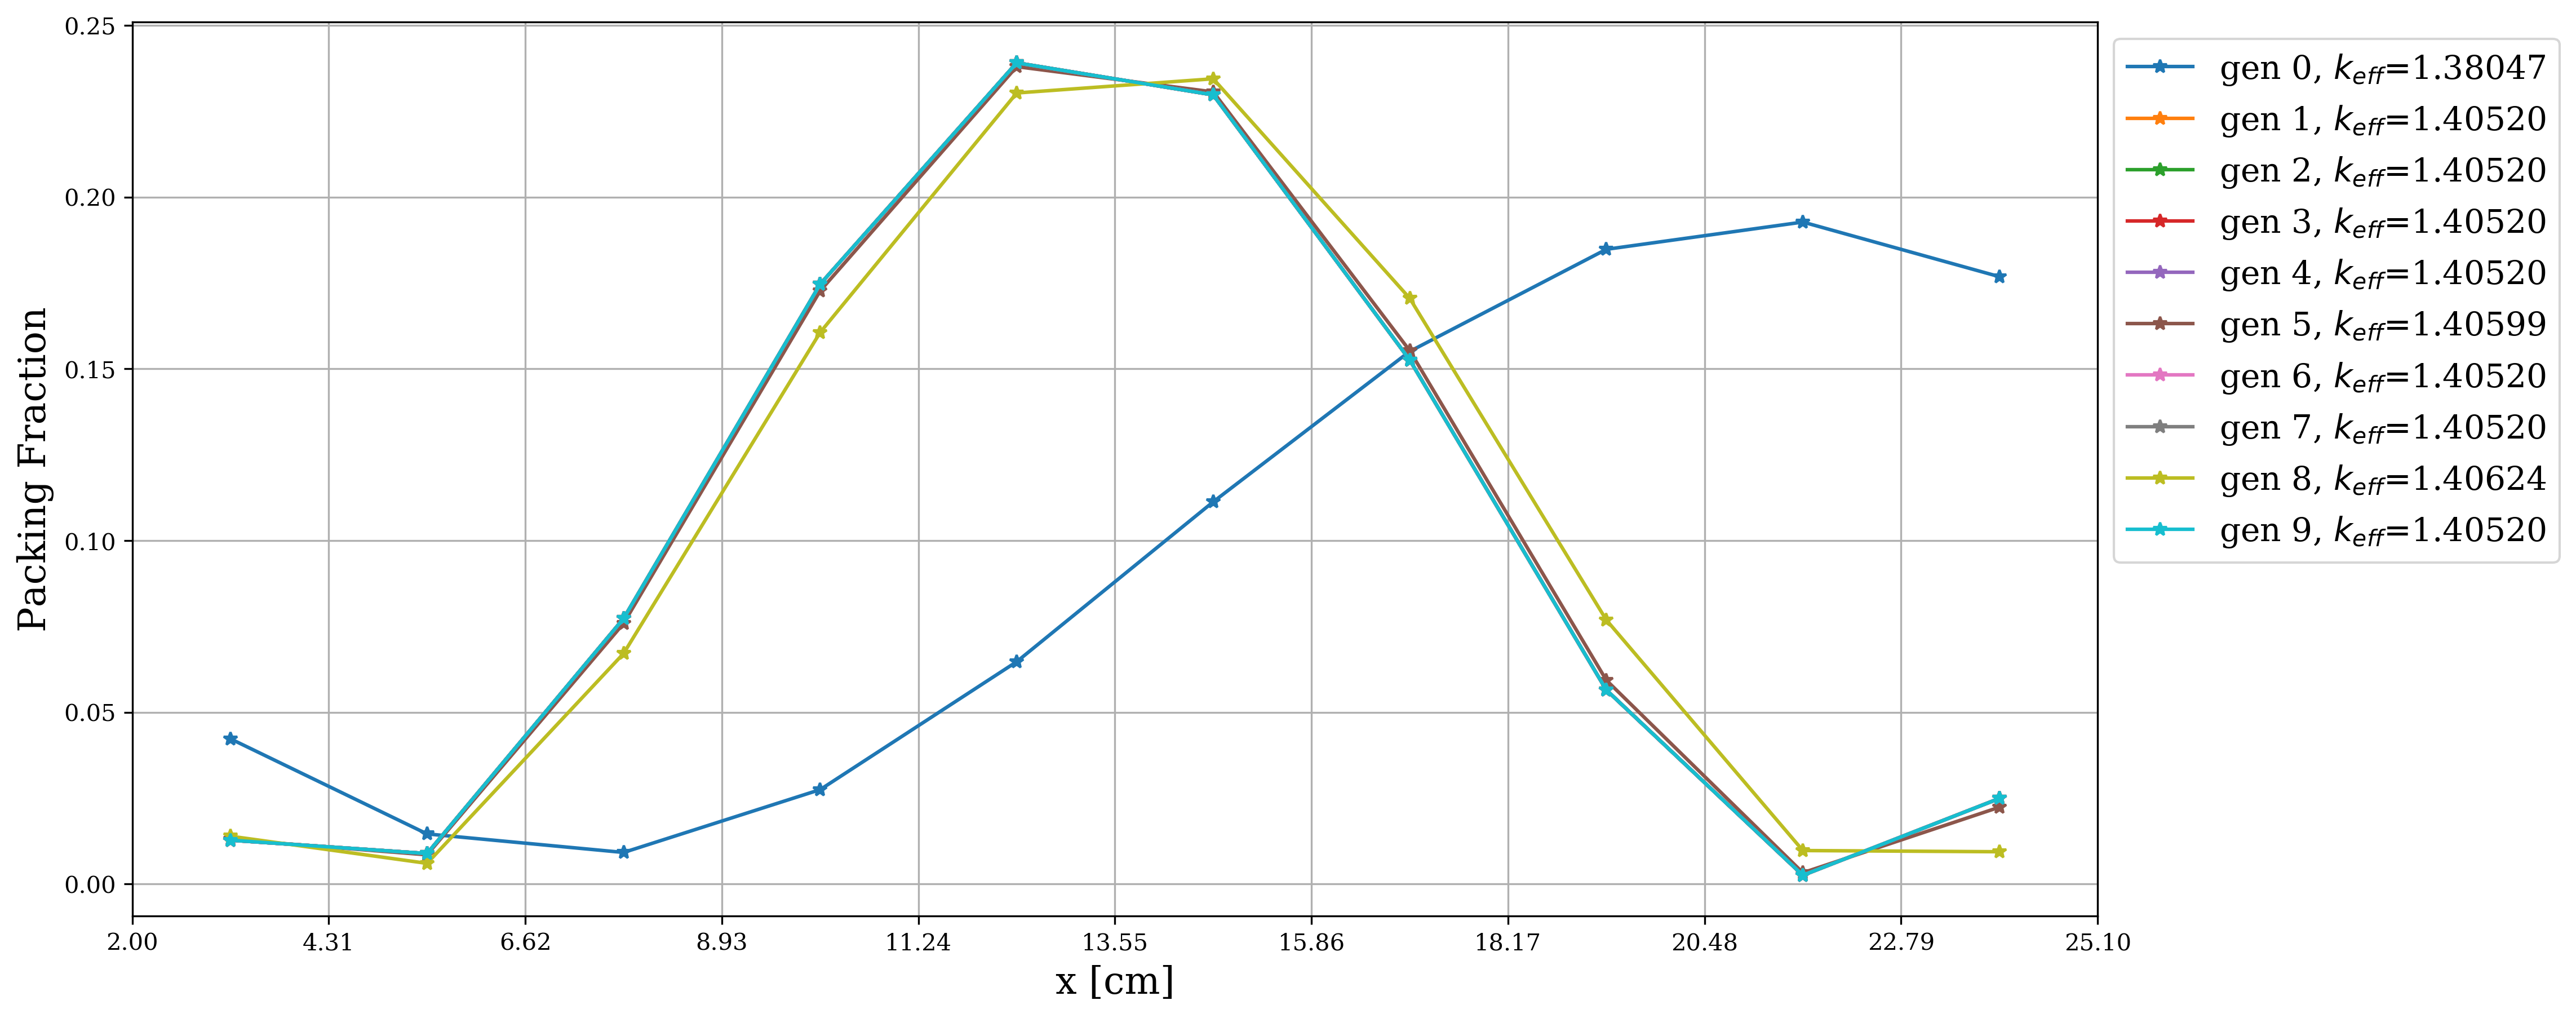
\includegraphics[width=1.1\linewidth]{pf_39.png}} 
        \caption{Maximum $k_{eff}$'s packing fraction distribution evolution.}
        \label{fig:pf_39}
    \end{subfigure}
    \caption{ Results for each generation for REALM's genetic algorithm optimization 
    of the Straightened \acrfull{AHTR} Fuel Slab. The REALM simulation used 
    the 39$^{th}$ experiment's hyperparameter set.}
    \label{fig:39}
\end{figure}
The maximum $k_{eff}$ converged quickly by generation 1, however, this is not 
usually the case. 
The genetic algorithm optimization process is stochastic, and so there is always 
the possibility that the algorithm randomly samples a set of input parameters
that maximizes the objective function early on in the genetic algorithm 
optimization process. 
The average $k_{eff}$ demonstrates how the average population of individuals converge 
towards a higher $k_{eff}$ with improvements from each generation. 
I used the BlueWaters supercomputer to run REALM. 

To demonstrate how the genetic algorithm optimization process usually goes, 
Figures \ref{fig:keff_conv_15} and \ref{fig:pf_15} show the evolution of $k_{eff}$ 
and packing fraction distribution through each generation of the second best 
performing 15$^{th}$ experiment, respectively. 
Experiment 15 demonstrates how both maximum and average $k_{eff}$ converges 
towards a higher $k_{eff}$ with improvements from each generation.
\begin{figure}[]
    \centering
    \begin{subfigure}{\textwidth}
    \makebox[\textwidth][c]{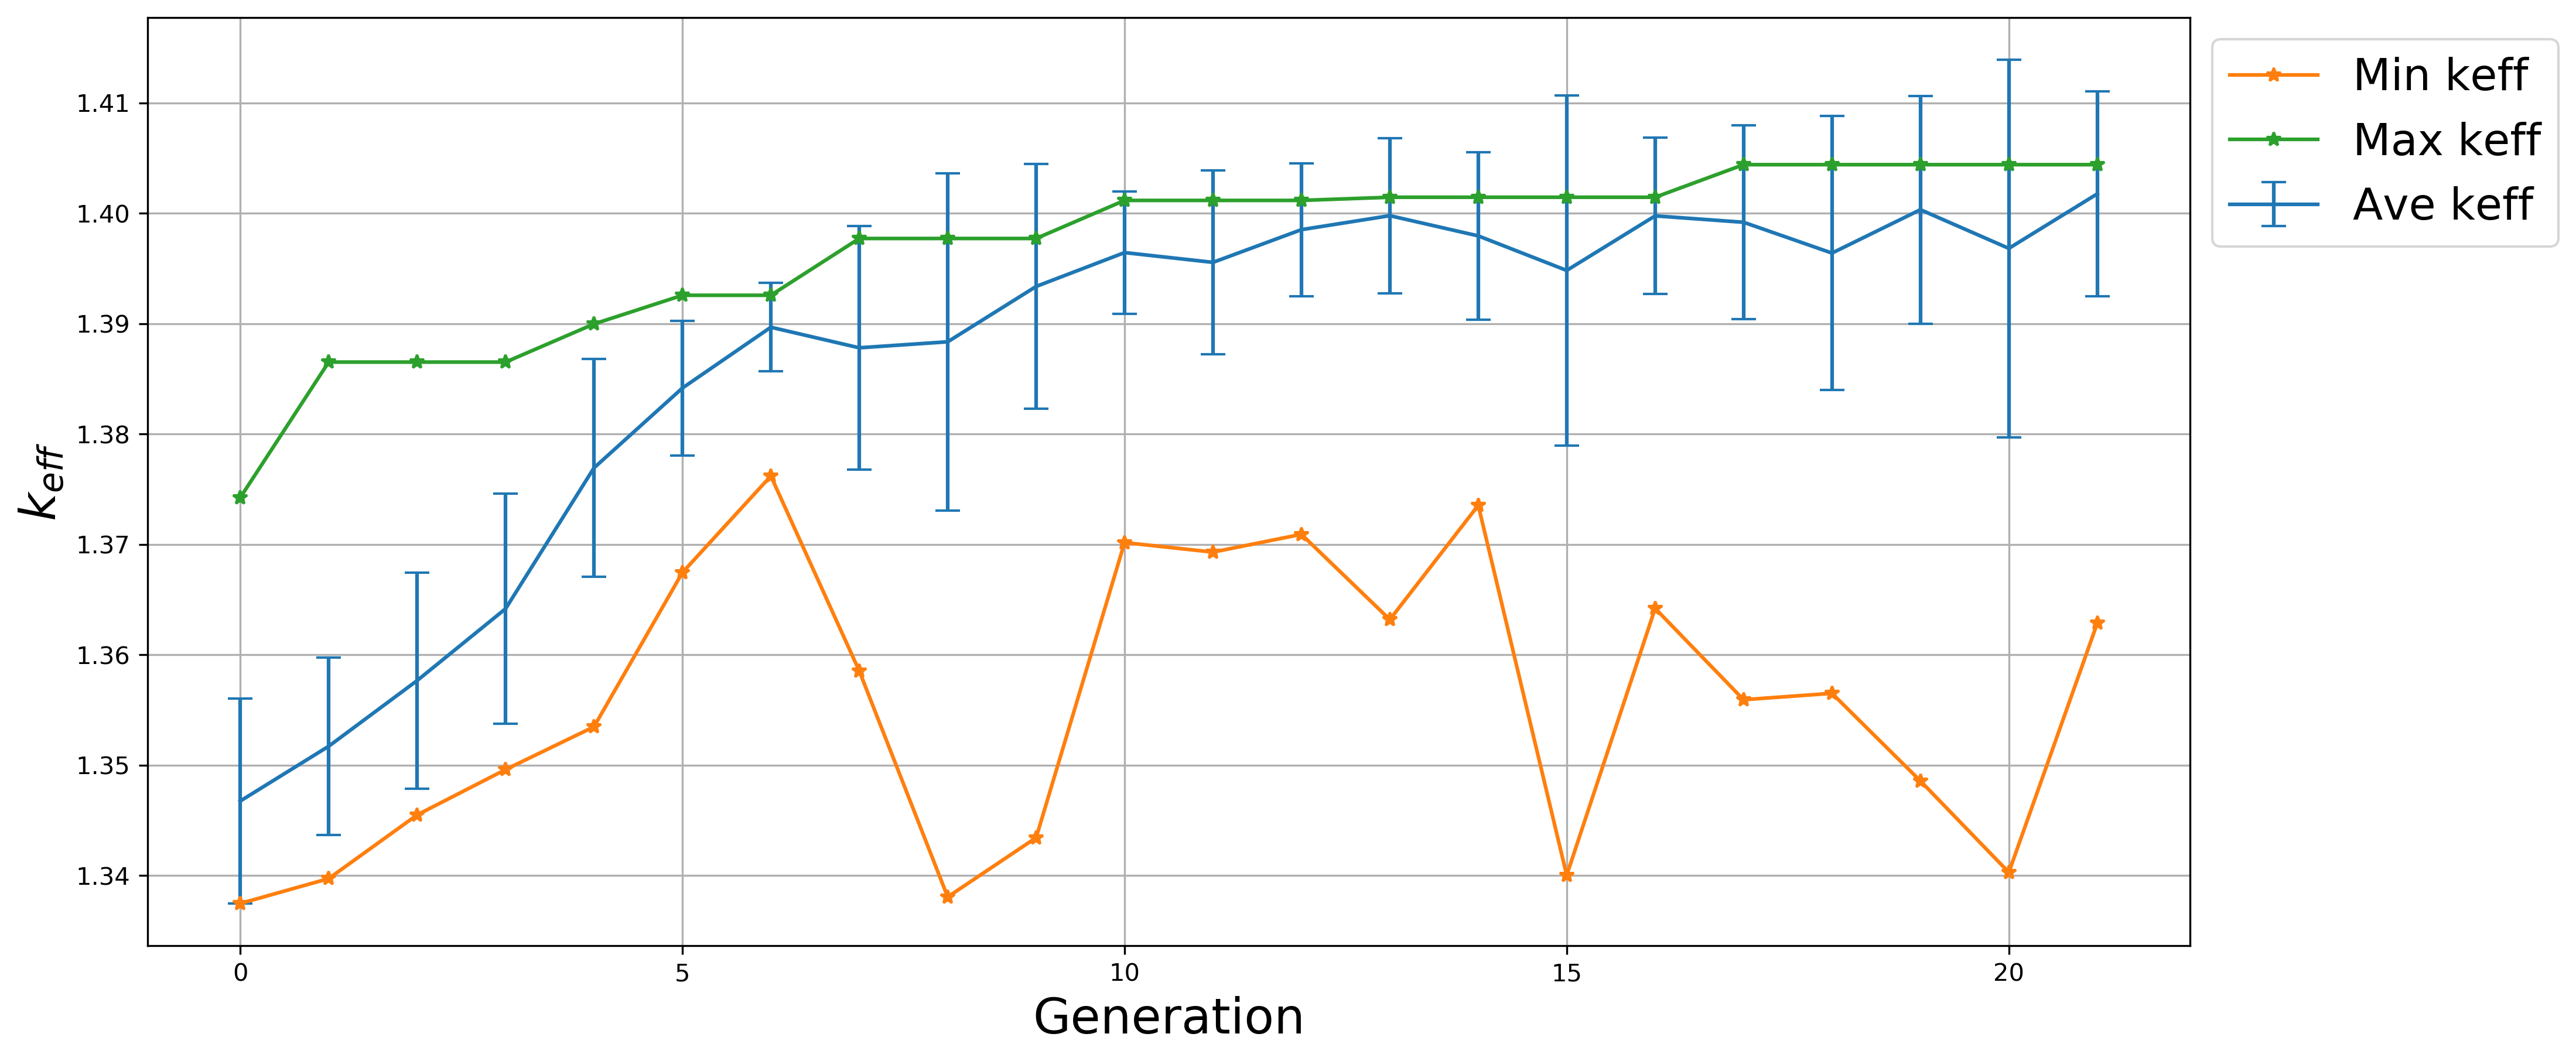
\includegraphics[width=1.1\linewidth]{keff_conv_15.png}} 
    \caption{Minimum, average, and maximum $k_{eff}$ values evolution.}
    \label{fig:keff_conv_15}
    \end{subfigure}
    \begin{subfigure}{\textwidth}
        \makebox[\textwidth][c]{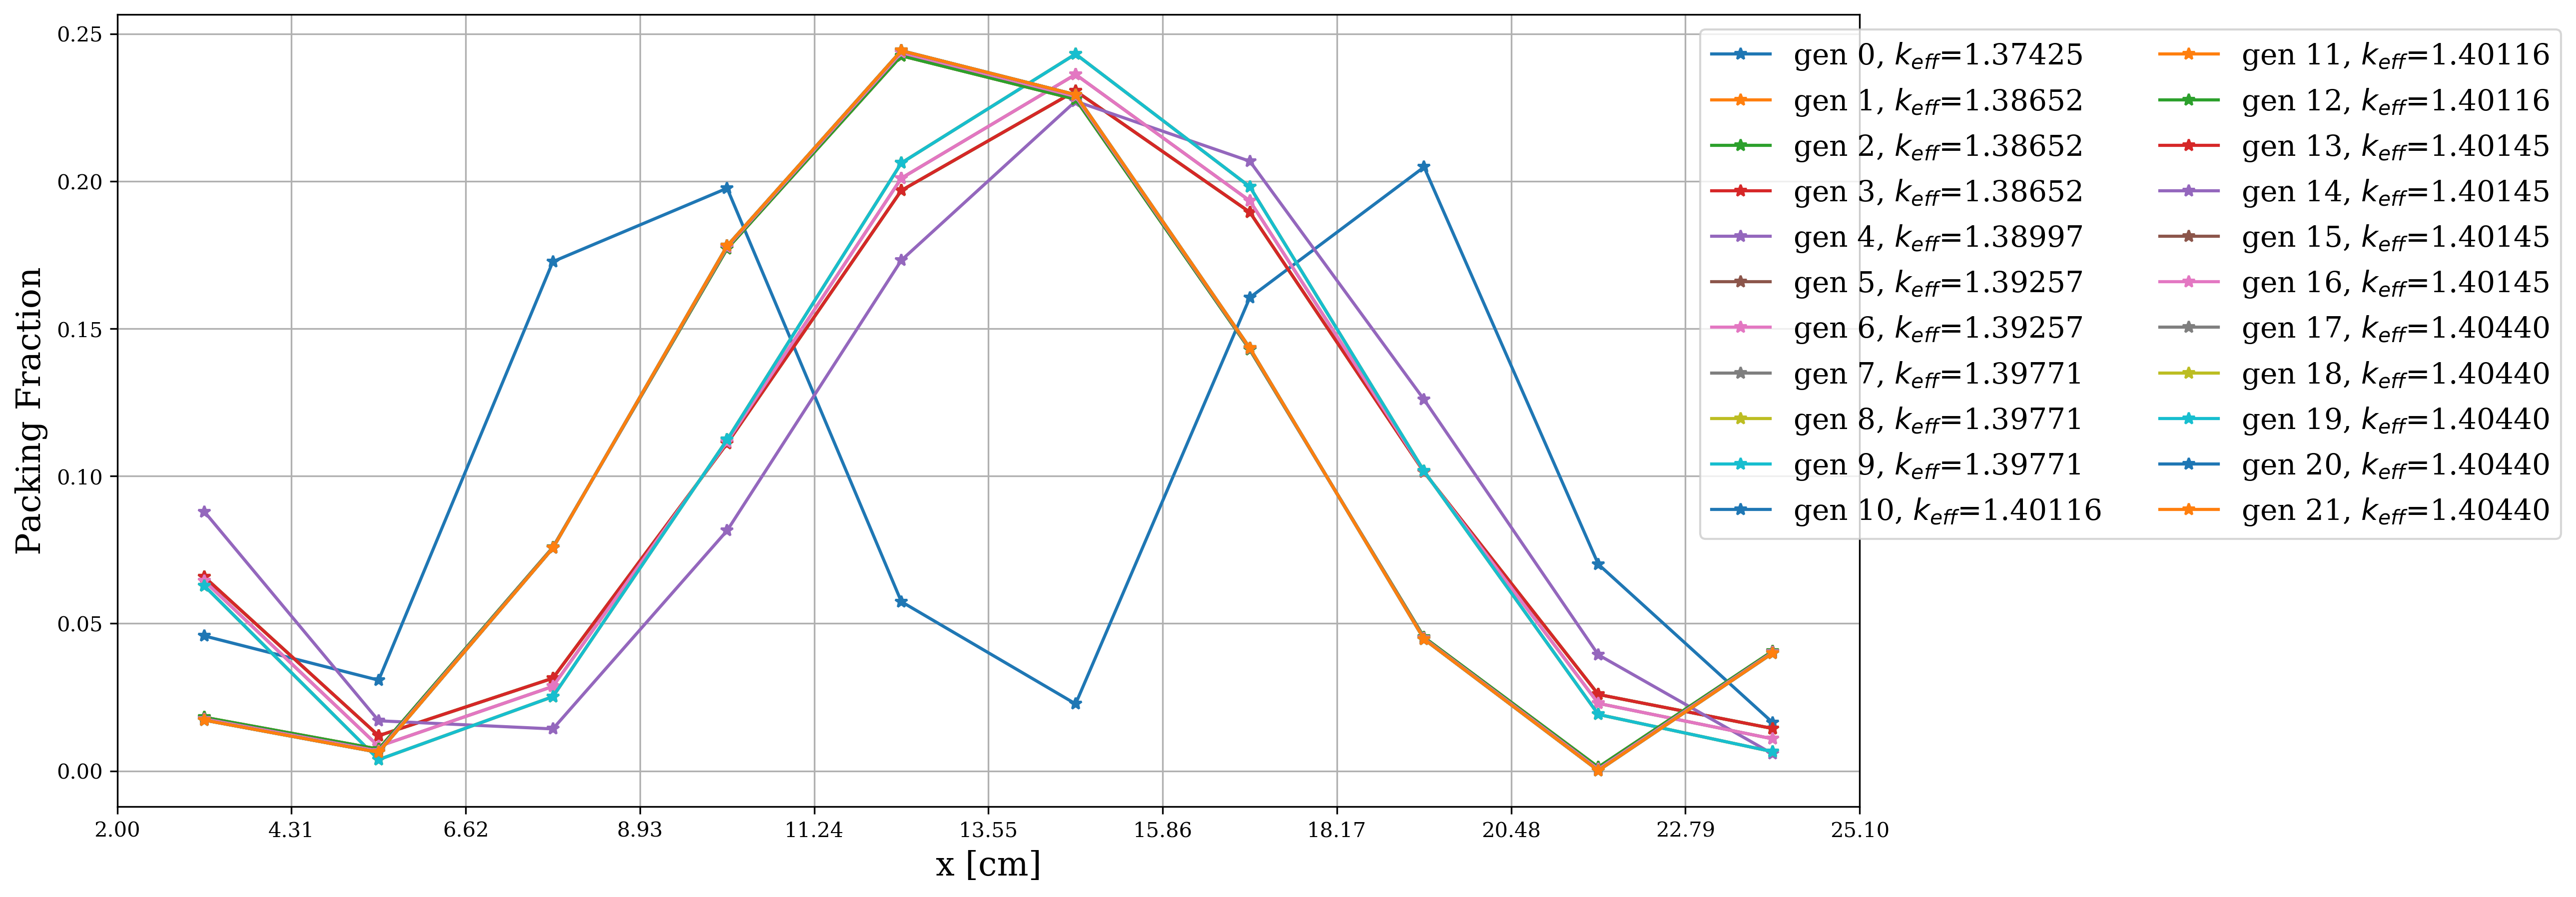
\includegraphics[width=1.1\linewidth]{pf_15.png}} 
        \caption{Maximum $k_{eff}$'s packing fraction distribution evolution.}
        \label{fig:pf_15}
    \end{subfigure}
    \caption{ Results for each generation for REALM's genetic algorithm optimization 
    of the Straightened \acrfull{AHTR} Fuel Slab. The REALM simulation used 
    the 15$^{th}$ experiment's hyperparameter set.}
    \label{fig:15}
\end{figure}

Both experiments 39 and 15 have packing fraction peaking at approximately 
0.23 in the centre of the slab and decreasing to zero at the sides of the slab.  
The amplitude, $a$, for the packing fraction distribution that produced $k_{eff max}$ 
for experiment 39 and the other top five experiments (Table \ref{tab:topfive}) 
have settled at the upper bound of approximately 2. 
This shows that a larger $k_{eff}$ occurs in the slab geometry with larger 
variations of packing fraction. 
These observations about packing fraction distribution for $k_{eff max}$ is 
consistent with what I understand from the original \gls{AHTR},: a high $k_{eff}$ 
occurs when there is a good balance between fuel loading and moderation space. 
Fission occurs at areas of high \gls{TRISO} particle concentration at thermal flux, 
however, the neutrons are born at fast flux and require moderation to slow down 
to thermal ranges.
Therefore, larger moderation areas ensure good resonance escape probability for 
the fast neutrons resulting in higher thermal flux, leading to more 
fission occurring and a higher $k_{eff}$. 

Another observation is that TRISO particles peak in the centre of the slab, 
proving that when only neutronics $k_{eff}$ is the objective function, the 
fuel tends to want to culminate in the middle. 
However, this is not ideal for heat transfer and ensuring flat power across 
the core. 

With these shortcomings in mind, I proceed to the future work chapter to discuss 
the types of simulations that will be run to optimize for these other parameters. 

% These ideas lead into the proposal section 

% IDEAS 
% vary in y direction 
% try the whole 1/3 diamond fuel elemt 

\section{Summary}
This chapter demonstrated applying \gls{REALM} to maximize $k_{eff}$ in a 
straightened \acrfull{AHTR} fuel slab through variation in the \gls{TRISO} 
particle packing fraction distribution. 
I began by conducting a coarse-to-fine random sampling hyperparameter search to 
find the genetic algorithm hyperparameters that worked best for this optimization 
problem.
Experiment 39 performed the best with a hyperparameter set that produced the 
highest final generation average $k_{eff}$ of 1.40165. 
The \gls{TRISO} particle packing fraction that produced the final generation's 
maximum $k_{eff}$ of 1.40519 peaks at the centre of the slab with a packing 
fraction distribution of $PF(x)=1.989\ sin(0.54x+3.143)$. 
This problem demonstrated how effective and robust genetic algorithms are for 
optimizing reactor parameters for an objective function. 
This demonstration problem had a single objective function which was to maximize 
$k_{eff}$. 
However, there are many other objectives that should be considered such as 
maximizing heat transfer, and minimizing power peaking in the core. 
Thus, in the next chapter, I will propose future simulations for optimizing
all these objective functions.
